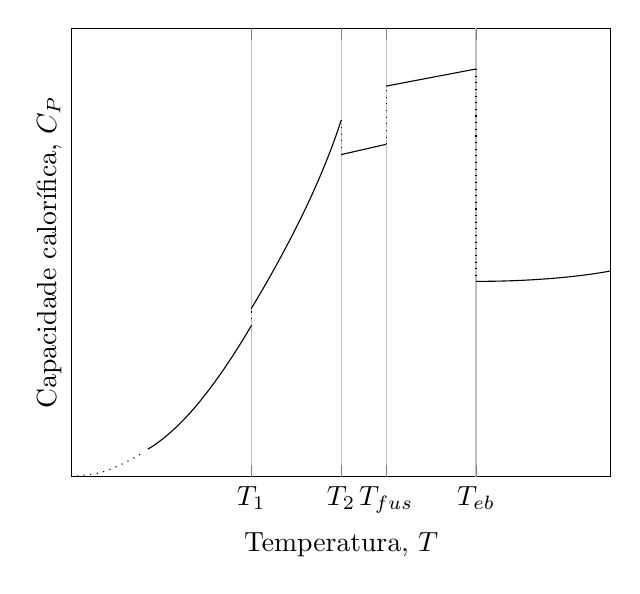
\begin{tikzpicture}
    \begin{axis}
        [
            xlabel = {Temperatura, $T$},
            ylabel = {Capacidade calorífica, $C_P$},
            ymin = 0.6, xmin = -16,
            xmin = 0, xmax = 120,
            xtick = \empty,
            ytick = \empty,
            extra x ticks = {40, 60, 70, 90},
            extra x tick labels={$T_1$, $T_2$, $T_\text{fus}$, $T_\text{eb}$},
            extra tick style={grid=major},
        ]
    \addplot [dotted, smooth] coordinates
        {
            (-12,0.5)
            (6,0.7)
            (16,1.3)
        };
    \addplot [smooth, tension=1] coordinates
        {
            (17,1.4)
            (28,2.7)
            (40,5)
        };
    \addplot [dotted] coordinates
        {
            (40,5)
            (40,5.5)
        };
    \addplot [smooth, tension=1] coordinates
        {
            (40,5.5)
            (52,8.4)
            (60,11)
        };
    \addplot [dotted] coordinates
        {
            (60,11)
            (60,10)
        };
    \addplot [black] coordinates
        {
            (60,10)
            (70,10.3)
        };
    \addplot [dotted] coordinates
        {
            (70,10.3)
            (70,12)
        };
    \addplot [tension=1] coordinates
        {
            (70,12)
            (90,12.5)
        };
    \addplot [dotted] coordinates
        {
            (90,12.5)
            (90,6.3)
        };
    \addplot [smooth, tension=1] coordinates
        {
            (90,6.3)
            (131,7)
            (140,9)
        };
    \end{axis}
    \end{tikzpicture}